

\documentclass[12pt]{article}
\usepackage{design_ASC}
\usepackage{graphicx}
\graphicspath{ {./images/} }
\usepackage{listings}
\setlength\parindent{0pt} %% Do not touch this

%% -----------------------------
%% TITLE
%% -----------------------------
\title{HomeWork 7} %% Assignment Title

\author{Dhirajsinh\\ %% Student name
RBE-595 - Optimal Control\\ %% Code and course name
\textsc{Worcester Polytechnic Institute }
}

\date{\today} %% Change "\today" by another date manually
%% -----------------------------
%% -----------------------------

%% %%%%%%%%%%%%%%%%%%%%%%%%%
\begin{document}
\setlength{\droptitle}{-5em}    
%% %%%%%%%%%%%%%%%%%%%%%%%%%
\maketitle

% --------------------------
% Start here
% --------------------------




\section*{}

{\bfseries The discrete approximation to a nonlinear continuous system is given by:\\ \\
$x(k + 1) = x(k) - 0.4x^2 (k) + u(k)$\\ \\
The state and control values are constrained by:\\ \\
$0 \leq x(k) \leq 1$\\ \\
$-0.4 \leq u(k) \leq 0.4$\\ \\
The performance measure to be minimized is:\\ \\
$ J = 4 \mid x(n+1) \mid + $\sum_{k=0}^{n} \mid u \mid $ $ \\

}



% %%%%%%%%%%%%%%%%%%%
\section*{Question 1}
% %%%%%%%%%%%%%%%%%%%
{Quantize the state into the levels 0, 0.5, 1, and the control into the levels -0.4, -0.2, 0, 0.2, 0.4.
Use any programming language (such as Matlab, Python, Java, C, ... ) to implement dynamic programming with linear interpolation to calculate J 1,2(x(1)) and J 0,2(x(0))}
\begin{tabular}{|l|l|}
\hline
x(1) & J 1,2(x(1)) \\ \hline
0.0  & 0.0         \\ \hline
0.5  & 0.4         \\ \hline
1.0  & 1.2         \\ \hline
\end{tabular}
\\
\begin{tabular}{|l|l|}
\hline
x(0) & J 1,2(x(0)) \\ \hline
0.0  & 0.0         \\ \hline
0.5  & 0.32        \\ \hline
1.0  & 0.52        \\ \hline
\end{tabular}

{\bfseries The code output is :\{0: \{0.0: 0.0, 0.5: 0.32, 1.0: 0.52\}, 1: \{0.0: 0.0, 0.5: 0.4, 1.0: 1.2\}\} \\}


\section*{Question 2}

{
Quantize the state into the levels 0, 0.002, 0.004, ..., 1, and the control into the levels -0.4,
-0.398, -0.396, ..., 0.4. Implement dynamic programming.\\
(a) Plot J* 1,2 as a function of x(1), and plot J* 0,2 as a function of x(0).\\
(b) Find the optimal control sequence u ∗ (0), u ∗ (1) and the minimum cost if the initial state
is 1.0.
}

\subsection*{Answer 2.a}


\begin{figure}[H]

\begin{subfigure}{}
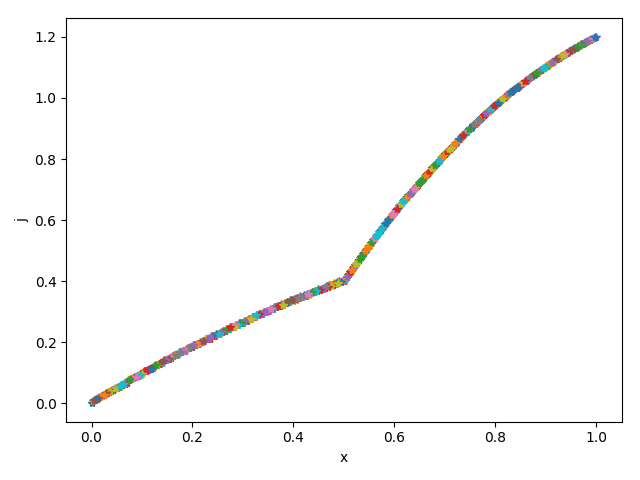
\includegraphics[width=10cm, height=7cm, centre]{2ax(1).png} 
\caption{Plot J* 1,2 as a function of x(1)}
\label{fig:subim1}
\end{subfigure}
\begin{subfigure}{}
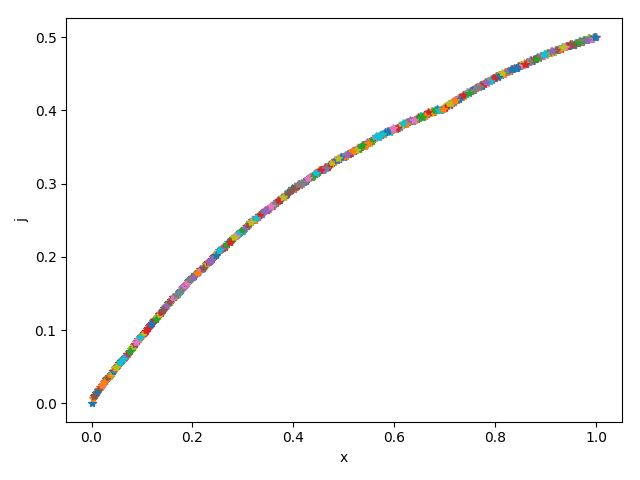
\includegraphics[width=10cm, height=7cm, centre]{2ax(0).png}
\caption{plot J* 0,2 as a function of x(0)}
\label{fig:subim2}
\end{subfigure}

\caption{cost vs state}
\label{fig:image2}
\end{figure}


\subsection*{Answer 2.b}

{
optimal control sequence u*(0), u*(1) and the minimum cost is : \\ 
initial state x(0) = 1   u= [-0.1, -0.4]\\
Cost of J 0,2(x(0)=1) = -0.1

}




\section*{Question 3}

{
Quantize the state into the levels 0, 0.002, 0.004, ..., 1, and the control into the levels -0.4,
-0.398, -0.396, ..., 0.4. Implement dynamic programming.\\ \\
(a) Plot J*0,20 as a function of x(0), plot J*1,20 as a function of x(1), plot J*18,20
as a function of x(18), and plot J*19,20 as a function of x(19). What do you observe about these figures?\\
(b) If the initial state is 1.0, find the minimum cost just using J*0,20 (not by calculating the optimal trajectory).\\
(c) Plot the optimal feedback control policy at step 19, which is u*(19), as a function of x(19), and plot the optimal feedback control policy at step 18, which is u*(18), as a function of x(18). What do you observe and can you guess why it occurs?\\
(d) If the initial state is 1.0, plot the optimal trajectory x*(k), k = 0, 1, ..., 20 as a function
of k, and plot the optimal control u*(k), k = 0, 1, ..., 19 as a function of k. Calculate the
performance measure J using the trajectory of x*and u*.J should be very close to your answer in (b). Otherwise, you may want to double check your code.\\


}



\subsection*{Answer 3.a}

{
\bfseries 
 System Dynamics :$x(k + 1) = x(k) - 0.4x^2 (k) + u(k)$\\ 
 Cost Function: $ J = 4 \mid x(20) \mid + $\sum_{k=0}^{19} \mid u \mid $ $ \\
 
As observed from the graphs below and given system dynamics,cost function we can infer that most of the cost function curves are flat and the values are close to zero for lower k (k=0,1) as system dynamics has nature of driving itself to origin without and control input (eg: K = Inf x(k)(approx) = 0,For all k, U= 0).\\

For cost curves for higher (k=18,19), the system cannot drive itself to origin without control input for higher state value and without control input it would result in higher terminal cost increasing cost function.\\

In graphs of k=18 there is sudden change in curve's nature at x(18)=0.8 which is due all states before 0.8 reach very close to origin without control input but states after 0.8 need some control effort to reduce high terminal cost.\\

Similarly in K=19 the graph shows sudden change in nature at k=19 as control effort reaches saturation and resulting high terminal cost.\\
}
\begin{figure}[H]

\begin{subfigure}{}
\centering
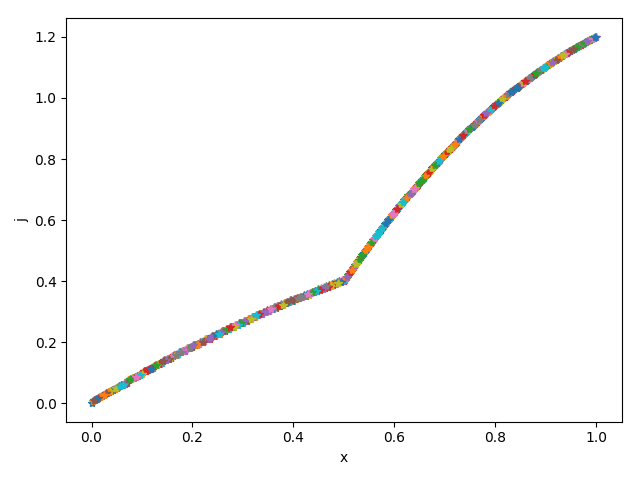
\includegraphics[width=10cm, height=8cm, centre]{3a19.png} 
\caption{Plot J* 19,20 as a function of x(19)}
\label{fig:subim1}
\end{subfigure}

\begin{subfigure}{}
\centering
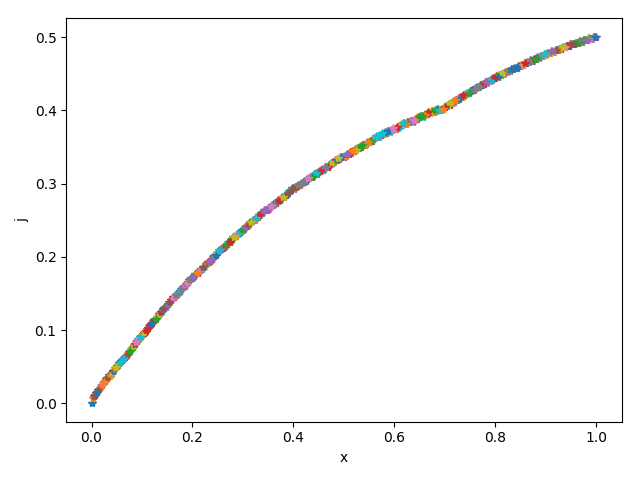
\includegraphics[width=10cm, height=8cm, centre]{3a18.png} 
\caption{Plot J* 18,20 as a function of x(18)}
\label{fig:subim1}
\end{subfigure}



\caption{cost vs state}
\label{fig:image2}
\end{figure}


\begin{figure}[H]

\begin{subfigure}{}
\centering
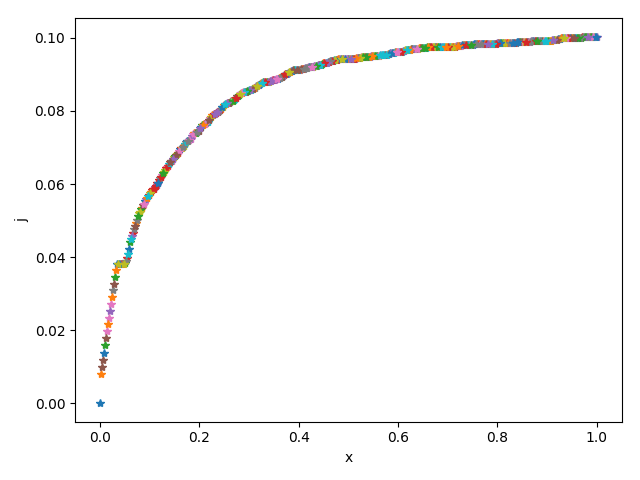
\includegraphics[width=10cm, height=8cm, centre]{3a1.png} 
\caption{Plot J* 1,20 as a function of x(1)}
\label{fig:subim1}
\end{subfigure}

\begin{subfigure}{}
\centering
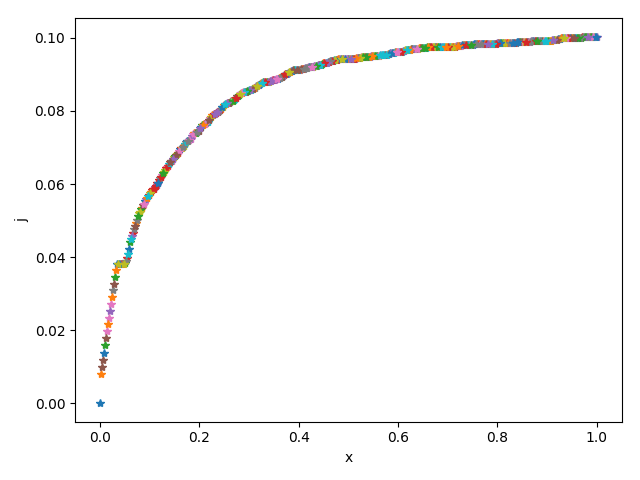
\includegraphics[width=10cm, height=8cm, centre]{3a0.png} 
\caption{Plot J* 0,20 as a function of x(0)}
\label{fig:subim1}
\end{subfigure}

\caption{cost vs state}
\label{fig:image2}
\end{figure}


\subsection*{Answer 3.b}

{
\bfseries Optimal Cost for initial state x(0)=1 from J*(0-20) is : 0.10028
}

\subsection*{Answer 3.c}

{\bfseries
As depicted in graph and system dynamics at most of the time step the control effort (U=0 at K=0,1) is zero as system drives itself to very close origin without any control input.\\

similarly at K=18 the system control effort is almost close to zero till x(18)=0.8 after which the control input increases to reduce terminal cost.\\

Similarly at K=19 the control input tries to drive the state to origin by increasing the control effort depending on current state of system but from graph after x(19)=0.5 the system cannot drive itself to origin as control efforts get saturated as it is bounded\\  

}

\begin{figure}[H]
\begin{subfigure}{}
\centering
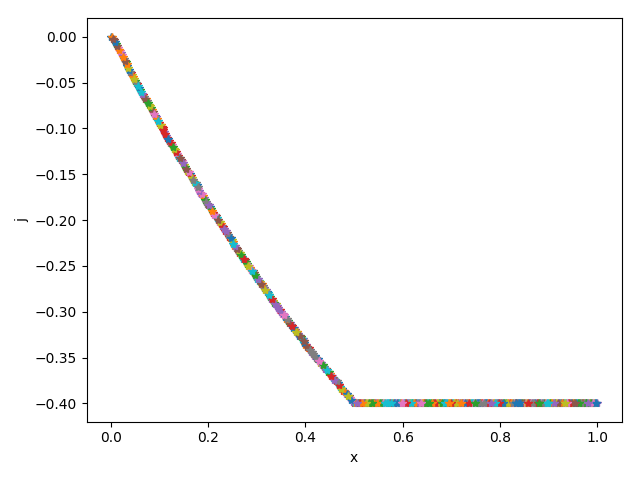
\includegraphics[width=10cm, height=6cm, centre]{3c19.png} 
\caption{Plot U* 19,20 as a function of x(19)}
\label{fig:subim1}
\end{subfigure}

\begin{subfigure}{}
\centering
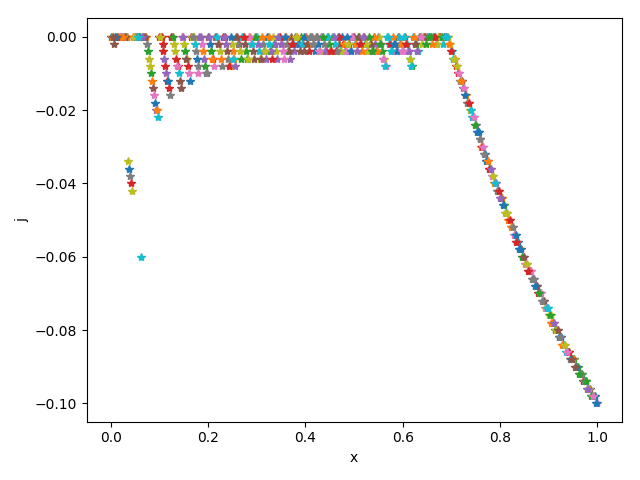
\includegraphics[width=10cm, height=6cm, centre]{3c18.png} 
\caption{Plot U* 18,20 as a function of x(18)}
\label{fig:subim1}
\end{subfigure}

\caption{Optimal Control vs state}
\label{fig:image2}
\end{figure}


\subsection*{Answer 3.d}

{
\bfseries Optimal cost using x* and u*  for intial state =1 is : 0.10021 \\
}

\begin{figure}[H]
\begin{subfigure}{}
\centering
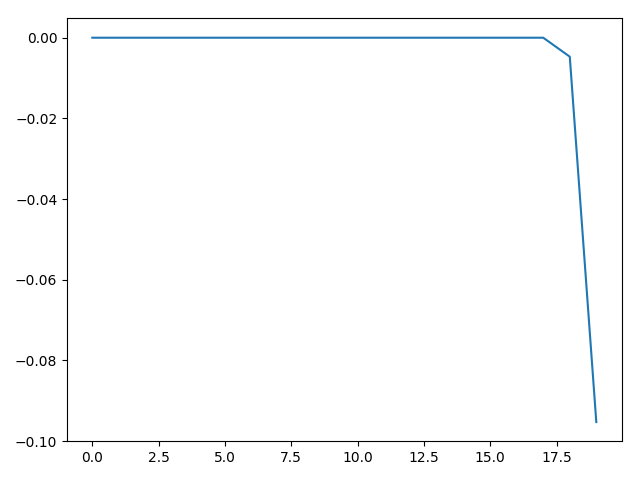
\includegraphics[width=10cm, height=8cm, centre]{3dkx.png} 
\caption{Plot X* vs K for X(0)=1}
\label{fig:subim1}
\end{subfigure}

\begin{subfigure}{}
\centering
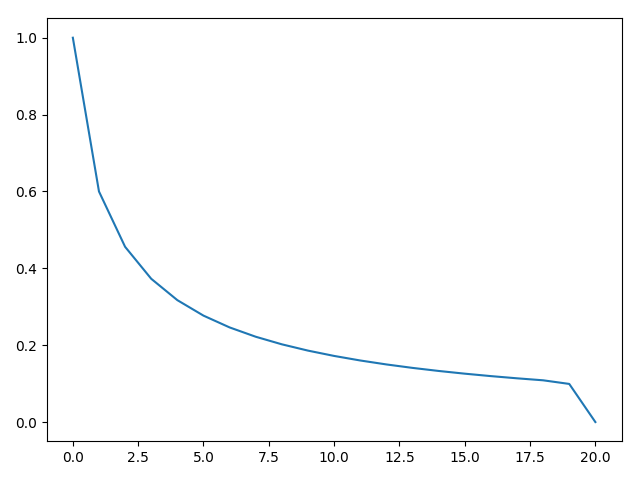
\includegraphics[width=10cm, height=8cm, centre]{3dku.png} 
\caption{Plot U* vs K for X(0)=1}
\label{fig:subim1}
\end{subfigure}

\caption{Optimal Control/State vs Time Step}
\label{fig:image2}
\end{figure}




\appendix
\section{Code}
 {
 \bfseries 
 Coded in Python using PyCharm IDE\\
 Library used: NumPy, Matplotlib, Collections \\
 Dynamic Programming**
 }

\section{Appendix 1 - Code for Question 1}

\begin{lstlisting}
import numpy as np
import matplotlib.pyplot as plt
from _collections import OrderedDict
states = list(map(lambda x : round(x,3),np.arange(0, 1.5, 0.5)))
controls = list(map(lambda x : round(x,3),np.arange(-0.4, 0.6, 0.2)))
new_st = []
dict=OrderedDict()
jj={}



def opt_con_cst():

    for i in states:
        dict[i]={}
        for j in controls:
            a= (i - (0.4*i*i) + j)
            if a<=1 and a>=0:
                dict[i][j]=round(a,3)


#
def optcost_st(step):
    a=step-1
    jj[a]={}
    if step == 2:
       for i in states:
           cost_cont=[]
           for u , x_next in dict[i].items():
               cost=4*x_next + abs(u)
               cost_cont.append(round(cost,3))
           jj[a][i]=min(cost_cont)
    else:
        for i in states:
            cost_cont = []
            for u, x_next in dict[i].items():
                cost = j_opt(round(x_next,3),step) + abs(u)
                cost_cont.append(round(cost,3))
            jj[a][i] = min(cost_cont)


def j_opt(x_nt,step):
    b=np.trunc(x_nt/0.5)
    a=(x_nt)-(b*0.5)
    if a==0:
       return jj[step][x_nt]

    else:
        m=(jj[step][round((b+1)*0.5,3)])
        n=(((x_nt-round((b+1)*0.5,3))/(round((b)*0.5,3)-round((b+1)*0.5,3))))
        l=((jj[step][round((b)*0.5,3)])-(jj[step][round((b+1)*0.5,3)]))

        return ((m)+(n*l))




if __name__ == "__main__":
    nstep=2
    opt_con_cst()


    for i in range(2,0,-1):
         optcost_st(i)

    print(jj)


\end{lstlisting}


\section{Appendix 2 - Code for Question 2 }

\begin{lstlisting}
import numpy as np
import matplotlib.pyplot as plt
from _collections import OrderedDict
states = list(map(lambda x : round(x,3),np.arange(0, 1.002, 0.002)))
controls = list(map(lambda x : round(x,3),np.arange(-0.4, 0.402, 0.002)))
new_st = []
dict=OrderedDict()
jj={}



def opt_con_cst():

    for i in states:
        dict[i]={}
        for j in controls:
            a= (i - (0.4*i*i) + j)
            if a<=1 and a>=0:
                dict[i][j]=round(a,5)


#
def optcost_st(step):
    a=step-1
    print(a)
    jj[a]={}
    if step == 2:
       for i in states:
           cost_cont=[]
           for u , x_next in dict[i].items():
               cost=4*x_next + abs(u)
               cost_cont.append([round(cost,3),u])
           jj[a][i]=min(cost_cont)
    else:
        for i in states:
            cost_cont = []
            for u, x_next in dict[i].items():
                cost = j_opt(round(x_next,3),step) + abs(u)
                cost_cont.append([cost,u])
            jj[a][i] = min(cost_cont)


def j_opt(x_nt,step):
    b=np.trunc(x_nt/0.002)
    a=(x_nt)-(b*0.002)
    if a==0:
       return jj[step][x_nt][0]

    else:
        m=(jj[step][round((b+1)*0.002,3)][0])
        n=(((x_nt-round((b+1)*0.002,3))/(round((b)*0.002,3)-round((b+1)*0.002,3))))
        l=((jj[step][round((b)*0.002,3)][0])-(jj[step][round((b+1)*0.002,3)][0]))

        return ((m)+(n*l))


def j_cont(x_nt,step):
    b=np.trunc(x_nt/0.002)
    a=(x_nt)-(b*0.002)
    if a==0:
       return jj[step][x_nt][1]

    else:
        m=(jj[step][round((b+1)*0.002,3)][1])
        n=(((x_nt-round((b+1)*0.002,3))/(round((b)*0.002,3)-round((b+1)*0.002,3))))
        l=((jj[step][round((b)*0.002,3)][1])-(jj[step][round((b+1)*0.002,3)][1]))

        return ((m)+(n*l))


if __name__ == "__main__":
    nstep=2
    opt_con_cst()

    for i in range(2,0,-1):
         optcost_st(i)

    #[print(jj[k]) for k in range(19,0,-1)]
    # print(jj[0][1])

    # question 2.a
    for pt in [0,1]:
        plt.figure()
        for key,value in jj[pt].items():


            plt.plot(key,value[0],'*')
            plt.xlabel("x")
            plt.ylabel("j")

    plt.show()

    # question 2.b
    u=[]
    initial_st=1
    for i in range(nstep):
        u.append(j_cont(initial_st,i))
        initial_st=(initial_st - (0.4*initial_st*initial_st) + u[i])

    print('initial state = 1   u=', u)
    print('Cost of J 0,2(x(0)=1) =',jj[0][1][1])


\end{lstlisting}


\section{Appendix 3 - Code for Question 3}

\begin{lstlisting}
import numpy as np
import matplotlib.pyplot as plt
from _collections import OrderedDict
states = list(map(lambda x : round(x,3),np.arange(0, 1.002, 0.002)))
controls = list(map(lambda x : round(x,3),np.arange(-0.4, 0.402, 0.002)))
new_st = []
dict=OrderedDict()
jj={}



def opt_con_cst():

    for i in states:
        dict[i]={}
        for j in controls:
            a= (i - (0.4*i*i) + j)
            if a<=1 and a>=0:
                dict[i][j]=round(a,5)


#
def optcost_st(step):
    a=step-1
    print(a)
    jj[a]={}
    if step == 20:
       for i in states:
           cost_cont=[]
           for u , x_next in dict[i].items():
               cost=4*x_next + abs(u)
               cost_cont.append([round(cost,5),u])
           jj[a][i]=min(cost_cont)
    else:
        for i in states:
            cost_cont = []
            for u, x_next in dict[i].items():
                cost = j_opt(round(x_next,3),step) + abs(u)
                cost_cont.append([round(cost,5),u])
            jj[a][i] = min(cost_cont)


def j_opt(x_nt,step):
    b=np.trunc(x_nt/0.002)
    a=(x_nt)-(b*0.002)
    if a==0:
       return jj[step][x_nt][0]

    else:
        m=(jj[step][round((b+1)*0.002,3)][0])
        n=(((x_nt-round((b+1)*0.002,3))/(round((b)*0.002,3)-round((b+1)*0.002,3))))
        l=((jj[step][round((b)*0.002,3)][0])-(jj[step][round((b+1)*0.002,3)][0]))

        return ((m)+(n*l))


def j_cont(x_nt,step):
    b=np.trunc(x_nt/0.002)
    a=(x_nt)-(b*0.002)
    if a==0:
       return jj[step][x_nt][1]

    else:
        m=(jj[step][round((b+1)*0.002,3)][1])
        n=(((x_nt-round((b+1)*0.002,3))/(round((b)*0.002,3)-round((b+1)*0.002,3))))
        l=((jj[step][round((b)*0.002,3)][1])-(jj[step][round((b+1)*0.002,3)][1]))

        return ((m)+(n*l))



if __name__ == "__main__":


    nstep=20
    opt_con_cst()

    for i in range(20,0,-1):
         optcost_st(i)

    #[print(jj[k]) for k in range(19,0,-1)]

    # question 3.a
    for pt in [0,1,18,19]:
        plt.figure()
        for key,value in jj[pt].items():


            plt.plot(key,value[0],'*')
            plt.xlabel("x")
            plt.ylabel("j")
    plt.show()

    # question 3.b
    print('cost for initial state =1 from j(0-20) is :',jj[0][1][0])

    # question 3.c
    for pt in [18,19]:
        plt.figure()
        for key,value in jj[pt].items():


            plt.plot(key,value[1],'*')
            plt.xlabel("x")
            plt.ylabel("j")

    plt.show()


    # question 3.d
    u=[]
    x=[]
    k1=np.arange(0,21,1)
    k2=np.arange(0, 20, 1)
    initial_st=1
    for i in range(nstep):
        x.append(round(initial_st,5))
        u.append(round(j_cont(initial_st,i),5))
        initial_st=(initial_st - (0.4*initial_st*initial_st) + u[i])
    x.append(round(initial_st, 5))
    l=sum(list(map(lambda y: abs(y) ,u)))
    cost=(4*x[20])+ l

    print('calculate cost using x* and u*  for intial state =1 is :',cost)

    plt.figure()
    plt.plot(k1,x)

    plt.figure()
    plt.plot(k2,u)

    plt.show()







\end{lstlisting}


\end{document}